\newpage
\section{Model Generation}
\hypertarget{sec:modelgen}
\genHeader


%\subsection{Generate model instances with TGGs}

In addition to model transformation and model synchronization, TGG specifications can be used to generate models. Often there is a need for large and randomly generated models for testing purposes. 
As creating large and valid models manually is quite difficult, eMoflon offers a model generation framework to automate this generation process. 



\begin{itemize}
\renewcommand\figurename{Figure}
\item[$\blacktriangleright$] Press the \texttt{new} button on the Eclipse toolbar and navigate to ``Examples/eMoflon Handbook Examples/''
(Fig.~\ref{eclipse:finalSolutionWizard}). Find and select \texttt{Final Solution : Visual} to copy the necessary projects into your workspace.

\vspace{0.5cm}

\begin{figure}[htbp]
\begin{center}
  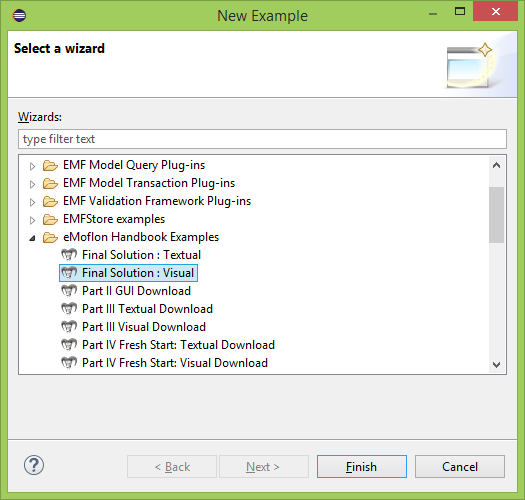
\includegraphics[width=0.8\textwidth]{eclipse_wizard_final.png}
  \caption{Get the final visual solution}
  \label{eclipse:finalSolutionWizard}
\end{center}
\end{figure}

\item[$\blacktriangleright$] Now delete the projects \texttt{Dictionary} and \texttt{DictionaryCodeAdapter} as they are not needed for the model generator. 
If successful, your workspace should resemble Fig.~\ref{eclipse:loadedDictionaryMetamodel}. 


\begin{figure}[htbp] 
\renewcommand\figurename{Figure}
\begin{center}
  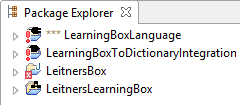
\includegraphics[width=0.5\textwidth]{eclipse_example_projects.png}
  \caption{Example projects from the wizard}
  \label{eclipse:loadedDictionaryMetamodel}
\end{center}
\end{figure}


\item[$\blacktriangleright$] In order to generate code for the model generator you should adjust your \textbf{moflon.properties.xmi} file in the \textbf{LearningBoxToDictionaryIntegration} project (Fig.~\ref{fig:moflon_properties_screenshot}).
Make sure that the value of the \textbf{TGG Build mode}
property is set to \textbf{SIMULTANEOUS} or \textbf{ALL} and save the file.


\begin{figure}[h]
\renewcommand\figurename{Figure}
\centering 
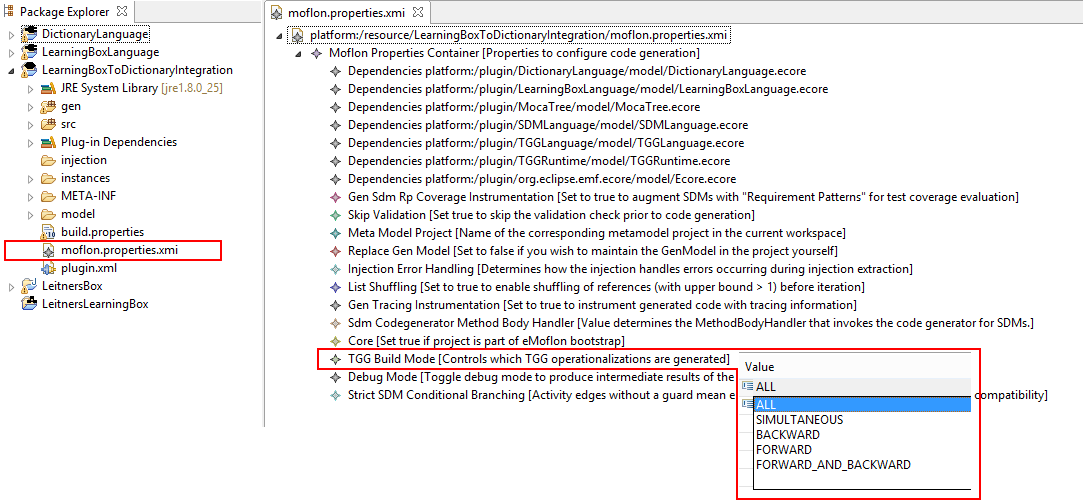
\includegraphics[width=1\textwidth]{moflon_properties_screenshot.png}
\caption{Screenshot of the \textbf{moflon.properties.xmi}}
\label{fig:moflon_properties_screenshot}
\end{figure}

\item[$\blacktriangleright$] Run a new \texttt{Export and build} on the \texttt{LeitnersLearningBox.eap} and build your projects in Eclipse in order to generate code. 


\end{itemize}
 
 

  
  
Now your generated code contains the necessary methods for model generation.
In your project \textbf{src} folder you can see the file
\textbf{LearningBoxToDictionaryIntegrationModelGen.java}
(Fig.~\ref{eclipse:modelgen}).
This class contains a stub and can be used to execute the model generation process.
 

 
\begin{figure}[htbp]
\renewcommand\figurename{Figure}
\begin{center}
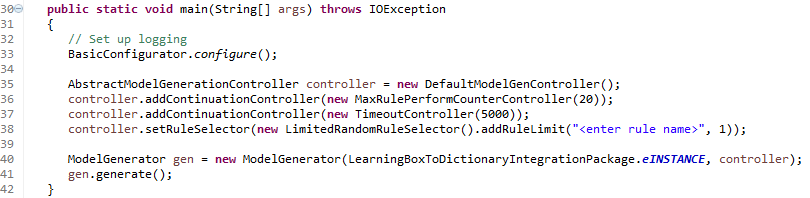
\includegraphics[width=1\textwidth]{eclipse_modelgen_stub.png}
\caption{Stub for the model generator}
\label{eclipse:modelgen}
\end{center}
\end{figure}

The \textbf{ModelGenerator} class uses an
\textbf{AbstractModelGenerationController} to control the generation process (line 35). In
this template the generation process will be terminated after 20 rules has been
performed (\textbf{MaxRulePerformCounterController} (line 36). 
Additionally, the \textbf{TimeoutController} will terminate the process after 5000ms (line 37). You can use the \textbf{MaxModelSizeController} class to terminate the generation process if
a specific model size has been reached. 
The \textbf{RuleSelector} controls which rules are selected as the next to be executed. 
The built-in \textbf{LimitedRandomRuleSelector} always selects a random rule and has the additional feature to limit the number of performs for specific rules (line 38).
For instance, if you want axiom rules to be performed exactly once to only generate models with a single root. 
You can create your own controller classes if the delivered ones are not sufficient. 
To create your first models do the following:


\begin{itemize}

\item[$\blacktriangleright$] Open your
\textbf{LearningBoxToDictionaryIntegrationModelGen.java} file.

\item[$\blacktriangleright$] Change \textbf{$<$enter rule name$>$} to \textbf{BoxToDictionaryRule} to
create single root models. This rule will only be performed once.

\item[$\blacktriangleright$] Save the file and run it.

\end{itemize}

You will get some logging information in the console (Fig.~\ref{eclipse:modelgen_log}) which contains
details gathered during the generation process such as model size for each domain, number of performs for
each rule, duration of generation process for each rule etc.


\begin{figure}[htbp]
\renewcommand\figurename{Figure} 
\begin{center}
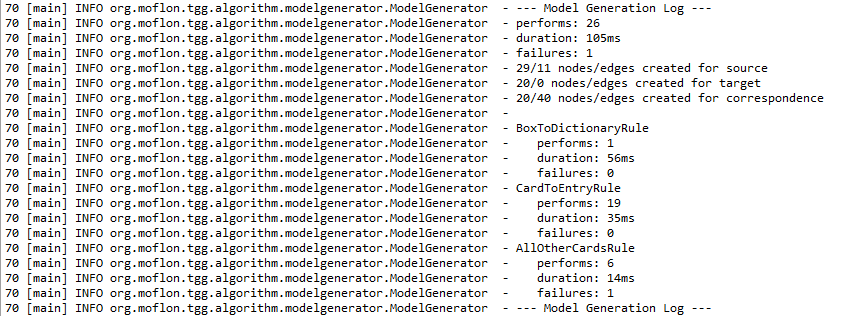
\includegraphics[width=1\textwidth]{eclipse_example_logging.png}
\caption{Logging output after model generation}
\label{eclipse:modelgen_log}
\end{center}
\end{figure}

In your \textbf{instances} folder should now be a new folder named
\textbf{generatedModels} with a timestamp suffix. It contains your newly generated
source and target models. \\



To support model generation for custom attribute constraints you may have to specify additional adornments. 
Adjusting the adornments is needed if the existing adornments does not cover the cases 
which arise using the TGG for model generation (e.g. the attribute constraints refers to only green object variables where all variables are free). 
Note that no additional adornments are required for our example.
\begin{itemize}

\item[$\blacktriangleright$] Open up the dialog for your custom constraint (figure \ref{fig:custom_constraint_definition}).

\item[$\blacktriangleright$] Enter the required adornments for the model
generator. Implement the new case in your constraint java
file. On figure \ref{eclipse:modelgen_eq_implementation} you can see the built-in implementation for the
\textbf{FF}-case of the \textbf{Eq}-constraint. The Generator class is able to
return random string values with respect to the type parameter. For a number
type the string will only contain numbers.

\end{itemize}

\begin{figure}[hbt] 
\centering 
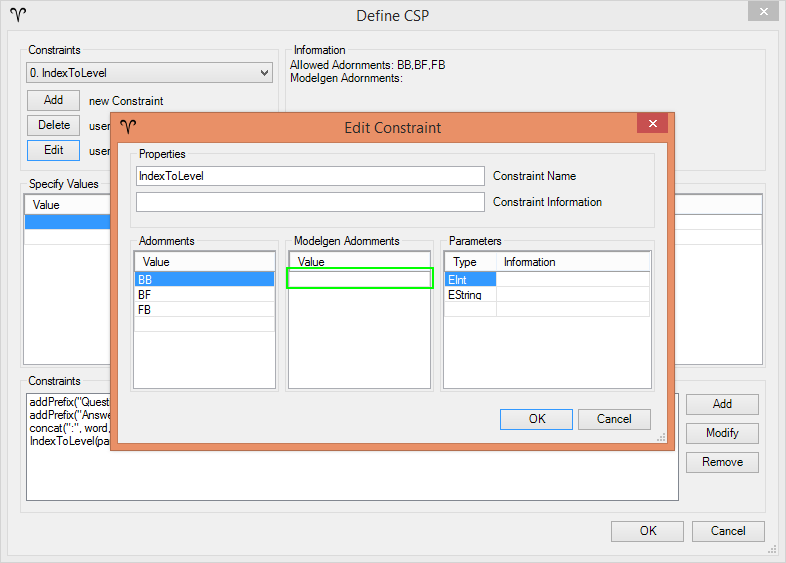
\includegraphics[width=1\textwidth]{custom_constraint.png}
\caption{Custom constraint dialog}
\label{fig:custom_constraint_definition}
\end{figure}
 


\begin{figure}[htbp]
\begin{center}
\begin{lstlisting}[language=Java,backgroundcolor=\color{white}, keywordstyle={\bfseries\color{purple}}]
// modelgen implementation
else if (bindingStates.equals("FF"))
{
  String value = Generator.getNewRandomString(a.getType());
  a.bindToValue(value);
  b.bindToValue(value);
  setSatisfied(true);
}
\end{lstlisting}
  \caption{Eq-constraint implementation for the FF case}
  \label{eclipse:modelgen_eq_implementation}
\end{center}
\end{figure}

 